%al posto di template.tex va messo il nome del file del livello superiore
\documentclass[../RiunioneInterna16-02-25.tex]{subfiles}

\begin{document}
\section{Verbale della riunione}		
	
\begin{itemize}

	\item Ad oggi il prototipo soddisfa quasi tutti i \textbf{requisiti obbligatori funzionali} fissati mentre mancano più del 50\% di \textbf{requisiti desiderabili funzionali}. Per questo è stata inviata una mail al proponente per modifica la priorità di alcuni requisiti da desiderabili a opzionali e altri da opzionali a desiderabili (mail \ref{fig:RichiestaMail}). Ricevuta la risposta affermativa (mail \ref{fig:RispostaMail}) dal proponente sono stati cambiati i seguenti requisiti da opzionali a desiderabili:
	\begin{itemize}
		\item ROpzF8.4.2.4;
		\item ROpzF8.4.2.5;
		\item ROpzF8.4.2.6;
		\item ROpzF10.2;
		\item ROpzF10.2.1;
		\item ROpzF10.2.2;
		\item ROpzF11;
		\item ROpzF11.1;
		\item ROpzF11.1.1;
		\item ROpzF11.1.1.1;
		\item ROpzF11.1.1.2;
		\item ROpzF12;
		\item ROpzF13.4;
		\item ROpzQ14;
	\end{itemize}
	
	I seguenti invece da desiderabili a opzionali:
	\begin{itemize}
		\item RDesF11.1.2.2;
		\item RDesF11.1.2.3;
		\item RDesF11.1.2.4;
		\item RDesF11.1.2.5;
		\item RDesF11.2.2.1;
		\item RDesF11.2.2.1.1;
		\item RDesP15;
	\end{itemize}
	Entro la fase attuale si punta a soddisfare e a raggiungere i 100\% dei requisiti obbligatori e desiderabili.
	

	\item Tutti i membri del team sono d'accordo nella decisione di non implementare nessun requisito opzionale e terminare i requisiti desiderabili funzionali prima del collaudo.

	
\end{itemize}


	
	\begin{figure} [h]
		
\includegraphics[width=\textwidth]{img/RichiestaMail}
		\caption{Mail inviata il 2016-05-24 dal gruppo Leaf al proponente}		
		\label{fig:RichiestaMail}
	\end{figure}
	\hfill
	\begin{figure}[h]
		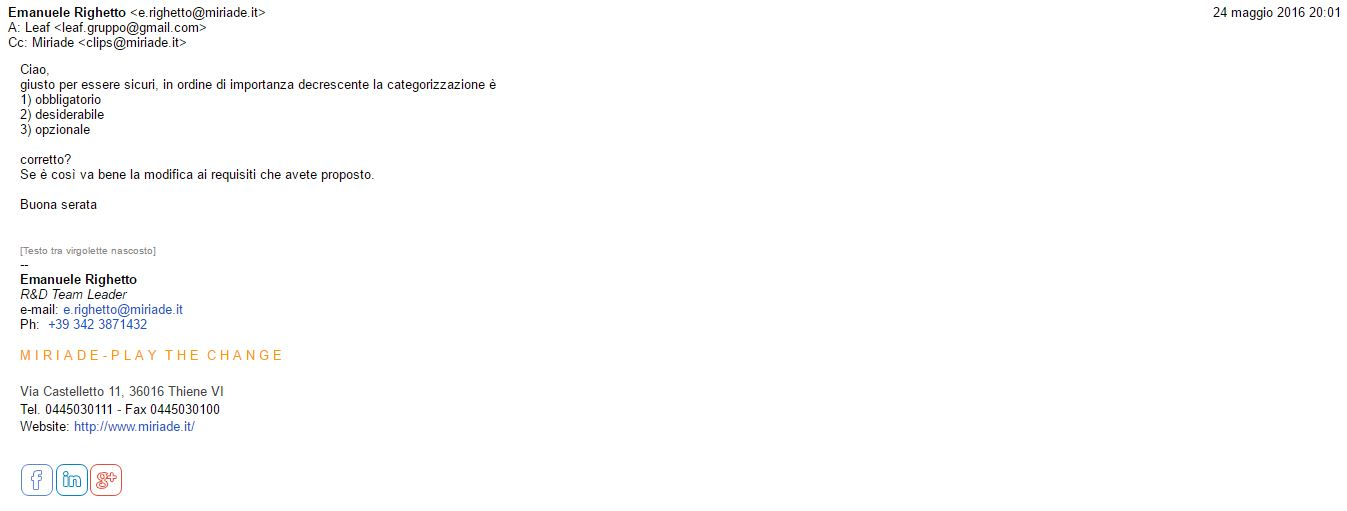
\includegraphics[width=\textwidth]{img/RispostaMail}
		\caption{Mail ricevuta il 2016-05-24 dal proponente in risposta alla mail precedente}		
		\label{fig:RispostaMail}
	\end{figure}

\end{document}

